\documentclass[12pt]{beamer}

\usepackage[english]{babel}
\usepackage{graphicx}
\usepackage[utf8]{inputenc}
\usepackage{tikz}

\usetheme{Copenhagen}

\title{Probability}
\author[Jacopo Notarstefano]{
    Jacopo Notarstefano\\
    \texttt{jacopo.notarstefano [at] gmail.com}
}
\date{11 February 2014}

\begin{document}
    \begin{frame}[plain]
        \titlepage
    \end{frame}

    \begin{frame}{Main ideas}
        \begin{enumerate}
            \item Given two pages, we want to estimate how many pages would be linked
            by both if links were created randomly.
            \item If the actual number is smaller, then we conclude that those pages
            are not related. If it's bigger, we assign a score between \(0\) and \(1\).
            \item This estimate depends on how we model random link creation between
            pages.
        \end{enumerate}
    \end{frame}

    \begin{frame}{The Barabási–Albert model}
    \end{frame}

    \begin{frame}{Balls and bins, 1/2}
        \begin{problem}
            Suppose that we have \(W\) bins, \(n_1\) red balls and \(n_2\) blue balls.
            When we throw a ball it falls in bin \(i\) with probability \(p_i\). When
            we are done throwing all the balls, what's the expected number of bins with
            both a blue and a red ball?
        \end{problem}
    \end{frame}

    \begin{frame}{Balls and bins, 2/2}
        \begin{solution}
            \textbf{If all throws are independent}, then, by linearity of expectation,
            we have
            \[
                \mathrm{E}[\vert N_1\cap N_2\vert] = \sum_{i,j=1}^{n_1,n_2}{\mathrm{E}[I_{ij}]} = n_{1}n_{2}\sum_{i=1}^{W}{p_{i}^2} = \mathbf{P}
            \]
            where 
        \end{solution}
    \end{frame}

    \begin{frame}{Results}
        \begin{figure}
            \makebox[\textwidth][c]{
                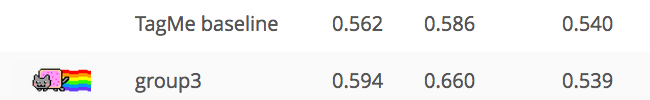
\includegraphics[scale=0.35]{tex/img/nyan}
            }
        \end{figure}
    \end{frame}
\end{document}
